%\section{Experiment}\label{exp}
We applied the proposed face recovering approach to three face databases to validate its accuracy. The three databases contain face images collected with different range sensors under various conditions such as lighting, poses, and expressions. The accuracy of reconstructed results is measured in terms of millimeters (mm), and is quantitatively evaluated by the mean absolute error (MAE)

\begin{align}
  e &= \frac{1}{n}\sum ^{n}_{i=1}\lvert D_r(i) - D_{gt}(i)\rvert
\end{align} 
, where $D_r$ is the reconstructed depth, $D_{gt}$ is the ground-truth, and $n$ is the total number of the facial points in the shape. 
To further eliminate errors caused by mis-aligned face images, the facial points are matched by applying iterative closest point method (ICP) \cite{besl1992method} before evaluating the mean absolute error. 
The Iterative Closest Point (ICP) algorithm is often used as an alternative approach aligning models. 
It could be used to not only reduce misalignment during the registration phase but also approximate the volume difference between two surfaces. 
However, it leads to problems with convergence when the initial misalignment of the data sets is large, and it need more computation time to align. 
To speed up ICP aligning process, we use $k$-dimensional tree to reduce nearest neighbor search time. 
After aligning, it can make sure two shapes in the same coordinate system and the facial features are aligned to the ground-truth shape. 
The estimated average error can better represent the actual reconstructed differences.

In this experiment, each image is divided into $8 \times 8$ overlapped patches with size of $15 \times 15$.
In the illustrations, our method is denoted by $Colortensor$. 
The selected color space is $YCbCr$ in the experiments. 
We also implemented three recently proposed methods \cite{reiter20063d}, denoted by $CCA$, which the images of grayscale image and depth are vectorized first and CCA is used to establish the relationship between the two data sets. 
The second method \cite{lei2008face}, which uses the NIR images and depth information mapping to tensor space, and learned the relationship between the two tensor spaces by CCA. 
In the experiments, grayscale images are substituted for NIR images in \cite{lei2008face}, and the results are denoted by $Graytensor$.
The third method \cite{lei2008face}, $Y$ images of the $YCbCr$ color space are substituted for NIR images, and the results are denoted by $Ytensor$.

The experimental results are shown in terms of the improvement ratio over the CCA method, which is defined as

\begin{align}
 \label{improvement}
 Percentage \, improvement = \frac{Err_{old} - Err_{new}}{Err_{old}} \times 100\%
\end{align} 
where $Err_{old}$ is obtained by CCA, and $Err_{new}$ is obtained by the proposed approach.

\section{Performance on Kinect-Generated Face Images}

The first image database is generated by taking 20 pairs of color and depth shots with Kinect. 
The images are taken in two environments: one with fixed lighting and the other with different lighting sources. 
A Microsoft LifeCam is used to capture photos and reconstruct 3D faces when generating the face image database by Kinect. 
%Because we want to reconstruct the 3D face just use a single color image. 
Once constructing the relationship between image and depth, we can use a single color image to recover the shape in the reconstruction phase. 
All faces are without accessories. 
In the training phase, database is randomly divided into disjoint training set and testing set,and each set contains 10 image pairs.

Figure \ref{fig:result01} and Figure \ref{fig:result02} show the reconstruction result on different split test sets under fixed lighting.
The corresponding accuracy is shown in Table \ref{table:Re1} and Table \ref{table:Re2}.
In Table \ref{table:Re1} and Table \ref{table:Re2}, each person shows two average errors, total pixels and facial features. 
Total pixels means the whole face. 
Facial features can be obtained by using facial features to compute convex hull which evaluates these points that have intersection between reconstruction result and ground-truth. 
In Table \ref{table:Re1}, each person shows the reconstruction errors, and the results of Colortensor are better than the results obtained by \cite{reiter20063d} and \cite{lei2008face}.
For comparison we show average reconstruction errors of the whole database by Kinect in Table \ref{table:Re1_2}.
It can be described that the uses of color image less sensitive to environmental lighting better than grayscale image as the 2D image.
In Figure \ref{fig:result01} and Figure \ref{fig:result02}, we show the reconstruction result under depth map and multiple views. 
The depth map is an image that contains information relating to the distance of the surfaces from a viewpoint. 
Depth map can make the depth range mapping to grayscale image as a single channel image.
According to depth map, we can determine the smoothness of reconstruction results .

Verifying the reconstruction shape still has better result than other methods under different lighting sources. 
The second environment is taking photos in the indoor environment, and using different direction office light. 
In Figure \ref{fig:result05} and Table \ref{table:Re2}, the input image is taken from different lighting, and our method still can get better result than other methods.
We also show average reconstruction errors of the whole database in Table \ref{table:Re2_2}. 
It is because that color information is considered in addition to the intensity information in the tensor construction, which causes the depth mapping be less sensitive to environmental lighting.  
 
\begin{table}[htbp]
\centering
\vfill 
\caption{Average reconstruction errors (mm) of different methods in different split test sets from our database by Kinect.}
\label{table:Re1}%
%\begin{tabular*}{\columnwidth}{@{\extracolsep{\fill}}|l||c|c|c|c|}
\begin{tabular}[b]{|l||c|c|c|c|c|c|c|}
% \begin{tabular}{|m{c}|m{c}|m{c}|m{c}|m{c}|m{c}|m{c}|}
\hline
 &  & CCA & Graytensor & improv.& Colortensor & improv. \\
\hline
\hline
 1  & Total  & 1.46 & 1.36 & 6.90\% & 1.33 & 8.30\%  \\   
    & Facial & 1.49 & 1.31 & 12.1\% & 1.29 & 13.3\%  \\ 

\hline
 2  & Total  & 1.49 & 1.43 & 4.61\% & 1.36 & 8.80\%  \\   
    & Facial & 1.52 & 1.37 & 9.60\% & 1.31 & 13.61\%  \\ 

\hline
 3  & Total  & 1.51 & 1.40 & 7.08\% & 1.37 & 9.26\%  \\   
    & Facial & 1.54 & 1.36 & 11.55\% & 1.32 & 13.72\%  \\ 


\hline
 4  & Total  & 1.38 & 1.35 & 1.98\% & 1.33 & 3.69\%  \\   
    & Facial & 1.34 & 1.30 & 2.70\% & 1.27 & 4.55\%  \\ 

\hline
 5  & Total  & 1.53 & 1.41 & 8.27\% & 1.36 & 9.35\%  \\   
    & Facial & 1.50 & 1.36 & 10.94\% & 1.31 & 11.93\%  \\ 

\hline
\end{tabular}%
\end{table}%

\begin{table}[htbp]
\centering
\vfill 
\caption{Average reconstruction errors (mm) of different methods from our database by Kinect.}
\label{table:Re1_2}%
%\begin{tabular*}{\columnwidth}{@{\extracolsep{\fill}}|l||c|c|c|c|}
\begin{tabular}[b]{|l||c|c|c|c|c|c|c|c|c|}
% \begin{tabular}{|m{c}|m{c}|m{c}|m{c}|m{c}|m{c}|m{c}|}

\hline
 &  & CCA & Graytensor & improv.& Ytensor & improv. &Colortensor & improv. \\
\hline
\hline
Avg. & Total  & 1.474 & 1.39 & 5.67\% & 1.40 & 5.02\% & 1.35 & 8.5\%  \\
     & Facial & 1.468 & 1.34 & 8.71\% & 1.36 & 7.35\% & 1.30 & 11.44\% \\
\hline

\end{tabular}
\end{table}%

\begin{table}[htbp]
\centering
\vfill 
\caption{Average reconstruction errors (mm) of different methods in different split test sets under different lighting source by Kinect.}
\label{table:Re2}%
%\begin{tabular*}{\columnwidth}{@{\extracolsep{\fill}}|l||c|c|c|c|}
\begin{tabular}[b]{|l||c|c|c|c|c|c|c|}
% \begin{tabular}{|m{c}|m{c}|m{c}|m{c}|m{c}|m{c}|m{c}|}
\hline
 &  & CCA & Graytensor & improv.& Colortensor & improv. \\
\hline
\hline
 1  & Total  & 1.45 & 1.43 & 1.37\% & 1.34 & 7.59\%  \\   
    & Facial & 1.43 & 1.38 & 3.49\% & 1.3 & 9.09\%  \\ 

\hline
 2  & Total  & 1.44 & 1.37 & 4.86\% & 1.32 & 8.33\%  \\   
    & Facial & 1.42 & 1.36 & 4.22\% & 1.31 & 7.74\%  \\ 

\hline
 3  & Total  & 1.47 & 1.38 & 6.12\% & 1.33 & 9.52\%  \\   
    & Facial & 1.52 & 1.36 & 10.52\% & 1.29 & 15.13\%  \\ 

\hline
 4  & Total  & 1.41 & 1.35 & 4.25\% & 1.31 & 7.8\%  \\   
    & Facial & 1.44 & 1.35 & 6.25\% & 1.30 & 9.72\%  \\ 
\hline
\end{tabular}%
\end{table}%

\begin{table}[htbp]
\centering
\vfill 
\caption{Average reconstruction errors (mm) of different methods under different lighting source by Kinect.}
\label{table:Re2_2}%
%\begin{tabular*}{\columnwidth}{@{\extracolsep{\fill}}|l||c|c|c|c|}
\begin{tabular}[b]{|l||c|c|c|c|c|c|c|c|c|}
% \begin{tabular}{|m{c}|m{c}|m{c}|m{c}|m{c}|m{c}|m{c}|}

\hline
 &  & CCA & Graytensor & improv.& Ytensor & improv. &Colortensor & improv. \\
\hline
\hline
Avg. & Total  & 1.443 & 1.39 & 3.67\% & 1.38 & 4.36\% & 1.35 & 8.5\%  \\
     & Facial & 1.453 & 1.36 & 6.4\%  & 1.33 & 8.46\% & 1.30 & 11.44\% \\
\hline

\end{tabular}
\end{table}%

\begin{figure*}
\begin{center}

  \includegraphics[scale=0.42]{figures/result01.eps}
  \caption{Shape recovery from a single color image by Kinect sensor}
  \label{fig:result01}

\end{center}
\end{figure*}


\begin{figure*}
\begin{center}

  \includegraphics[scale=0.38]{figures/result02.eps}
  \caption{Shape recovery from a single color image by Kinect sensor}
  \label{fig:result02}

\end{center}
\end{figure*}


\begin{figure*}
\begin{center}

  \includegraphics[scale=0.38]{figures/result05.eps}
  \caption{Shape recovery from a single color image by Kinect sensor under different lighting source}
  \label{fig:result05}

\end{center}
\end{figure*}
 
\section{Performance on CASIA 3D Face Database}

 \begin{figure}[htbp]
\centering 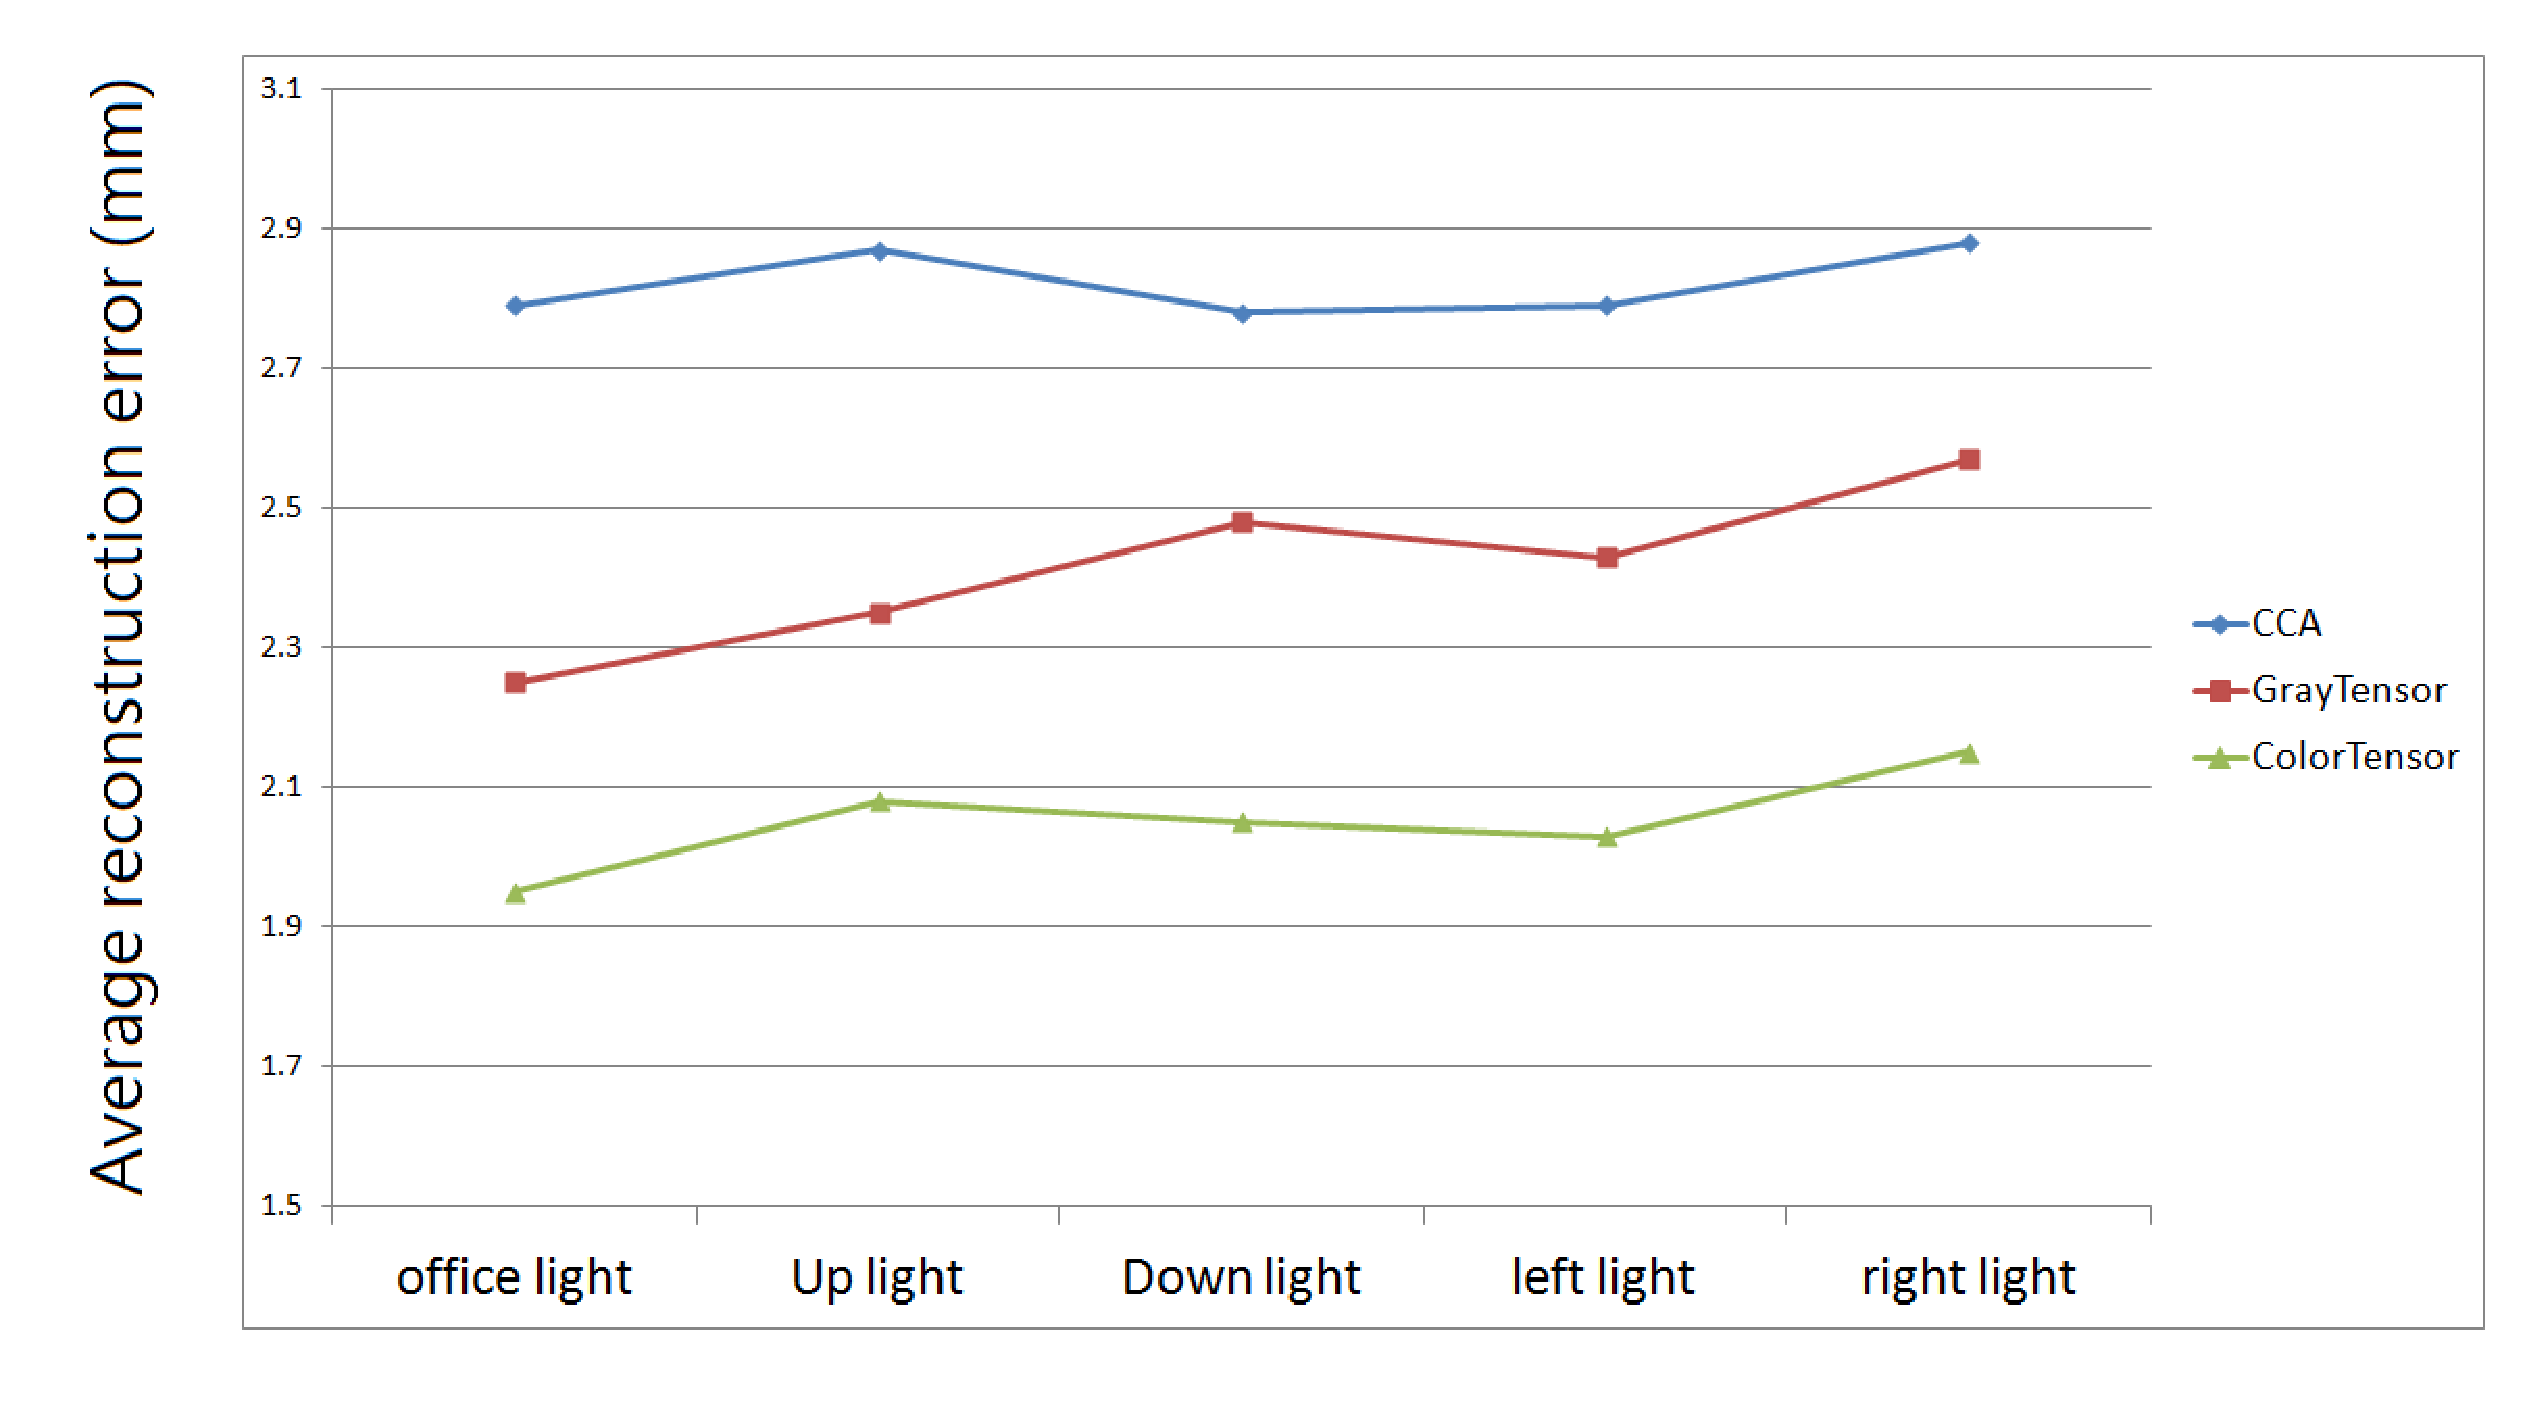
\includegraphics[%
  width=12cm]{figures/pic1.eps}
\caption{3D reconstruction error of different degrees on different method.}
\label{fig:multi-degree}
\end{figure}

\begin{figure}[htbp]
\centering 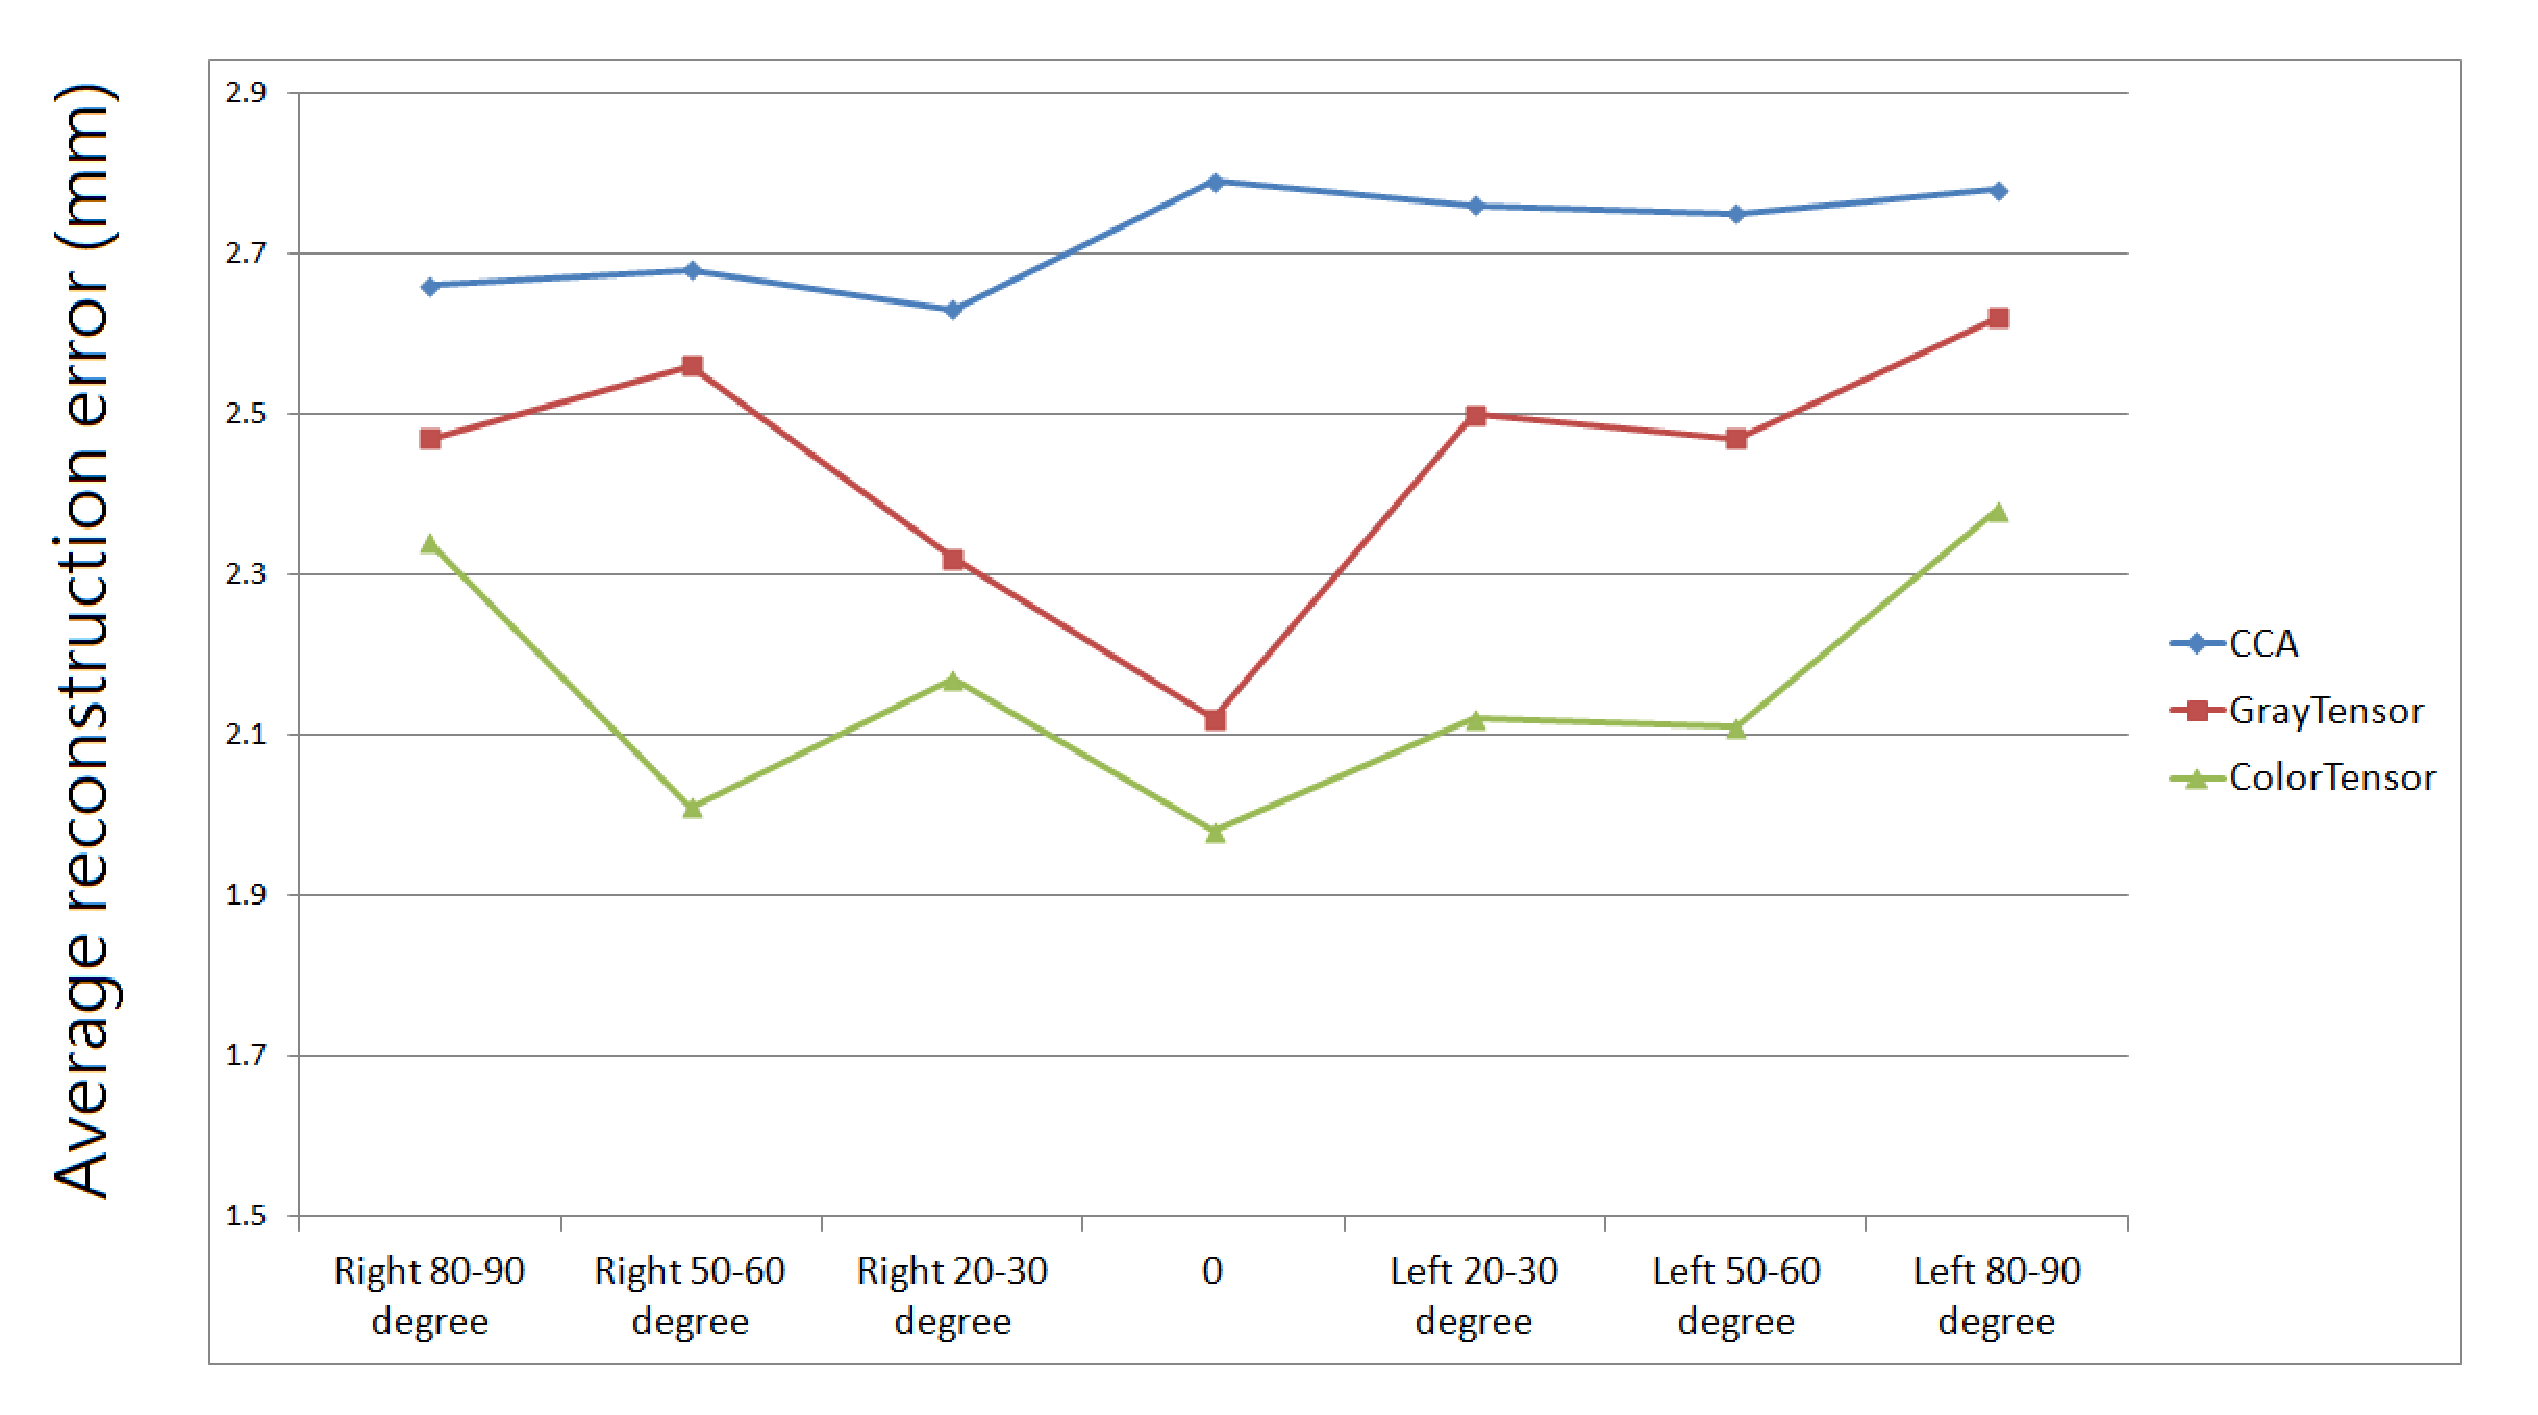
\includegraphics[%
  width=12cm]{figures/pic2.eps}
\caption{3D reconstruction error of different lighting on different method.}
\label{fig:multi-lighting}
\end{figure}

We applied the proposed approach to another face image database, CASIA 3D Face \cite{CASIA-3DFaceV1}, which contains images of 123 people (96 men and 27 women).
The images were taken under various environmental conditions, such as illuminations, expressions and poses by Minolta Vivid 910. 
In this database, there are not only the single variations of poses, expressions and illuminations, but also the combined variations of expressions under illuminations and poses under expressions. 
To verify our method, we can work in different illuminations conditions. We have several experiments in different environmental lighting. 
In the training phase, database is also divided into training set and testing set randomly. 
Training set contains 60 pairs of persons, and testing set includes the remaining 63 pairs of persons.

%In the CASIA 3D face database, it combined variations of expressions under different light sources and different poses.
We conducted two sets of experiments: one uses different viewpoints from the same person and the other uses the frontal face images with different lighting sources.
The results show that our method not only can reconstruct the front faces but also can deal with face images with different poses.
Samples of the reconstructed faces are shown in Figure \ref{fig:multi-degree} and Figure \ref{fig:multi-lighting}.
In Figure \ref{fig:multi-degree}, we randomly choose 10 persons from the CASIA 3D face database, and each person has different poses to recover face shape. 
After recovering, we align these shapes through ICP algorithm and compute the average reconstruction error of different poses. 
In different poses, our method has better results than other methods. It can verify that the color image is less sensitive to environmental lighting than the grayscale image under different poses. 
The second environment is under different lighting sources from the same front face image. 
In Figure \ref{fig:multi-lighting}, we randomly choose 10 persons and compute the average reconstruction errors. 
Our method has the minimal reconstruction errors than other methods.
When lighting sources change strongly, other methods for reconstruction errors are rapidly increasing.
In Figure \ref{fig:multi-lighting}, the average error of our reconstruction results is always about 2 mm. 
Because in these diverse lighting source environments, each person's grayscale image has a huge difference. 
This result can be ascribed to the use of color image instead of grayscale image, and can get better reconstruction shape in different environments.


In the Table \ref{table:Re3} shows the reconstruction result on different split test sets from CASIA 3D face database. 
The reconstruction results are shown in the Figure \ref{fig:result03}. 
In Figure \ref{fig:result03}, it shows that only use of a single color image to reconstruct. 
For comparison we show average reconstruction errors of the whole CASIA 3D face database in Table \ref{table:Re3_2}.
We also provide the ground truth and our results to compare. 
Each person shows the front pose image, depth map, and different views. 
The depth map is using the same depth range for ground truth and reconstruction results. 
In the depth map of reconstruction results, it still has some noisy points inside. 
Especially, in the fifth person, we have used interpolation algorithm to fill holes before computing tensor analysis. 
The reconstruction result can get more natural of model face than of original data. 


\begin{table}[htbp]
\centering
\vfill 
\caption{Average reconstruction errors (mm) of different methods in different split test sets from CASIA 3D face database.}
\label{table:Re3}%
%\begin{tabular}[b]{|c||c|c|c|c|c|c|}
\begin{tabular}[b]{|l||c|c|c|c|c|}
% \begin{tabular}{|m{c}|m{c}|m{c}|m{c}|m{c}|m{c}|m{c}|}
\hline
 &  CCA & Graytensor & improv. & Colortensor & improv.\\
\hline
\hline
 1  & 2.69 & 2.47 & 16.59\% & 2.12 & 21.05\%  \\   
\hline
 2  & 2.69 & 2.44 & 9.24\% & 2.21 & 17.88\%   \\
\hline
 3  & 2.51 & 2.38 & 5.03\% & 2.02 & 12.36\%   \\
\hline
 4  & 2.67 & 2.38 & 10.09\% & 2.14 & 19.74\%   \\
\hline
\end{tabular}%
\end{table}%


\begin{table}[htbp]
\centering
\vfill 
\caption{Average reconstruction errors (mm) of different methods from CASIA 3D face database.}
\label{table:Re3_2}%
%\begin{tabular*}{\columnwidth}{@{\extracolsep{\fill}}|l||c|c|c|c|}
\begin{tabular}[b]{|l||c|c|c|c|c|c|c|c|c|}
% \begin{tabular}{|m{c}|m{c}|m{c}|m{c}|m{c}|m{c}|m{c}|}

\hline
     & CCA & Graytensor & improv.& Ytensor & improv. &Colortensor & improv. \\
\hline
\hline
Avg. & 2.64 & 2.42 & 8.33\% & 2.36 & 10.6\% & 2.168 & 17.8\%  \\

\hline

\end{tabular}
\end{table}%



\begin{figure*}
\begin{center}

  \includegraphics[scale=0.42]{figures/result03.eps}
  \caption{Shape recovery from a single color image by the proposed method}
  \label{fig:result03}

\end{center}
\end{figure*}


\begin{figure*}
\begin{center}

  \includegraphics[scale=0.38]{figures/result04.eps}
  \caption{Shape recovery from a single color image by different methods}
  \label{fig:result04}

\end{center}
\end{figure*}


\section{Performance on Texas 3D Face Database}

The third database is the Texas 3D Face Recognition (Texas 3DFR) database \cite{gupta2010anthropometric,gupta2010texas,Texas3DFace} which is a collection of 1149 pairs of facial color and range images of 118 adult human subjects. 
This database can provide images which have very high spatial resolution of the $x$, $y$, and $z$ dimensions by using a stereo imaging system. 
Each $z$ value is represented in an 8 bit format with the highest value of 255 assigned to the tip of nose and the background assigned to the value of 0.
We can get accurate depth information from range image, and color image as input in our experiment. 
In the training phase, we also separate this database into training set and testing set randomly. 
In this experiment, we randomly choose two men and women from testing set to recover face shape. 
In Figure \ref{fig:result06} and Table \ref{table:Re4}, we can observe that our method has smaller average error than Graytensor, and in the multiple views can show our reconstructions are smoother. 
We also show average reconstruction errors of the whole Texas 3D face database in Table \ref{table:Re4_2}.

\input{tables/table4.tex}

\begin{figure*}
\begin{center}

  \includegraphics[scale=0.38]{figures/result06.eps}
  \caption{Shape recovery from a single color image by different methods from Texas 3D         Database}
  \label{fig:result06}

\end{center}
\end{figure*}

\section{Discussion}

In the indoor environment, there are many office light and others lighting sources. 
These factors may cause some problems like difference among grayscale images, and the environmental lighting is dissimilar when taking photo each time. 
To solve these problems, we propose a reconstruction algorithm which increases multiple factors like color information in tensor model of image and 3D space, and it can get a better relationship between color image and 3D depth image. 
We have different experiments while changing lighting source to verify our method as well. 
In the reconstruction phase, the color image is less sensitive than the grayscale image while changing lighting sources. 
It can be described that the discrepancy between color images are minor under different strength and direction lighting sources. 


